

%==============================================================================
%==============================================================================
\chapter{ {\cal HomCont} Demo : Homoclinic branch switching.} \label{ch:HomCont_hbs}
%==============================================================================
%==============================================================================

%==============================================================================
%DEMO=hbs======================================================================
%==============================================================================

This demo illustrates homoclinic branch switching, which is an
implementation of Lin's method \cite{Li:90,Sa:93,Ye:01}
as described in \citeasnoun{OlChKr:02}. We use a
direct branch switching method to switch from 1- to 2- and
3-homoclinic orbits near an inclination flip bifurcation 
in a model due to Sandstede, 
which was introduced in Chapter~\ref{ch:HomCont_san}.
This also shows how to obtain a homoclinic orbit through continuation
of a periodic orbit born at a Hopf bifurcation.
Thereafter, we illustrate homoclinic branch switching for the
FitzHugh-Nagumo equations and a 5th-order Korteweg-De Vries model.

\section{ Branch switching at an inclination flip in Sand\-stede's
  model.}
\label{sec:HomCont_hbs_san}
Consider the system \cite{Sa:95b}
\begin{equation} \begin{array}{rcl}
\dot{x} & = & a x + b y - a x^2 - \alpha z x (2-3x), \\
\dot{y} & = & b x + a y - \frac{3}{2} x (b x + a y) + \alpha z 2 y, \\
\dot{z} & = & c z + \mu x + 3 x z + \alpha (x^2 (1-x) - y^2).
\end{array} \end{equation}
as given in the file \filef{ sib.c}, where for simplicity we have
set $\tilde\mu=0$, $\beta=1$ and $\gamma=3$.

We study an inclination flip that exists for $a=0.375$,
$b=0.625$ and $c=-0.75$. This corresponds to the situation
where the eigenvalues of the equilibrium at the origin are
$a+b=1$, $a-b=-0.25$ and $c=-0.75$. Hence, the corresponding
bifurcation diagram consists of a complicated structure involving a
fan of infinitely many $n$-periodic and $n$-homoclinic orbits
for arbitrary $n$ and a region with horseshoe dynamics; see
also \citeasnoun{HoKr:00} and the references therein.

This computation starts from an equilibrium at $(2/3,0,0)$, which
exists for $a=\mu=\alpha=0$. Also, $b$ is set to $0.625$ (the value
we would like it to be) and $c$ is set to $-2.5$ in \funcf{stpnt}.
Choosing $c=-2$ at this stage leads to convergence problems.
This equilibrium is not the one corresponding to the homoclinic orbit,
but it is an equilibrium with complex eigenvalues, that we can follow
until it reaches a Hopf bifurcation. A periodic orbit emanates from 
this Hopf bifurcation and can be followed to the homoclinic orbit.
However, first we need to change $a$ from $0$ to $0.375$.

All the following commands, except for \commandf{demo('sib')}
are contained within the file \commandf{'sib.auto'} which you can 
either execute in a batch mode by entering\\
\commandf{> auto sib.auto}\\
or step by step using\\
\commandf{AUTO> demofile('sib.auto')}.

We start by copying the demo to the current work directory 
and running the first step
\begin{center}
\commandf{ demo('sib') }\\
\commandf{ ld('sib') } \\
\commandf{ rn() } \\
\commandf{ sv('1') }
\end{center}
The equilibrium is followed in $a$ until $a$ (or \parf{ PAR(1)}) is at our
desired value, $0.375$.
\begin{verbatim}
  BR    PT  TY LAB    PAR(1)     ...     U(1)          U(2)          U(3)     
   1     1  EP   1  0.000000E+00 ... 6.666667E-01  0.000000E+00  0.000000E+00
   1     6  EP   2  3.750000E-01 ... 6.666667E-01 -1.333333E-01  0.000000E+00
\end{verbatim}
The output is saved in the files \filef{ b.1}, \filef{ s.1} and
\filef{ d.1}.
Next we continue in $\alpha$ (\parf{PAR(4)}) until a Hopf bifurcation is
found:
\begin{center}
\commandf{ rn(c='sib.2',s='1') }\\
\commandf{ sv('2') }
\end{center}
or, alternatively,
\begin{center}
\commandf{ cc("IRS",2) }\\
\commandf{ cc("ICP",[4]) }\\
\commandf{ rn(s='1') }\\
\commandf{ sv('2') }
\end{center}
\begin{verbatim}
  BR    PT  TY LAB    PAR(4)     ...    U(1)          U(2)          U(3)     
   1    18  HB   3  3.184290E-01 ... 6.543750E-01 -1.347543E-01  7.701025E-02
\end{verbatim}
The output is saved in the files \filef{ b.2}, \filef{ s.2} and
\filef{ d.2}.
This Hopf bifurcation can then be continued into a periodic orbit. The
periodic orbit eventually reaches a homoclinic bifurcation. We
continue in $\mu$=\parf{PAR(5)} and \parf{PAR(10)}, 
which corresponds to the period, and stop when the period is equal to $35$.
\begin{center}
\commandf{ rn(c='sib.3',s='2') } \\
\commandf{ sv('3') }
\end{center}
\begin{verbatim}
  BR    PT  TY LAB    PAR(5)        L2-NORM     ...    PERIOD    
   3     5       5 -2.418809E-03  6.705689E-01  ...  1.089749E+01
                                                ...
   3    40       8 -1.294950E-02  6.145469E-01  ...  1.412970E+01
                                                ...
   3    81  EP  13 -1.046566E-04  4.018291E-01  ...  3.499999E+01
\end{verbatim}
The output is saved in the files \filef{ b.3}, \filef{ s.3} and
\filef{ d.3}. Note that $\mu$ first decreases and then increases towards
$0$, which is precisely what we expect in this model, as homoclinic
orbits occur on the line $\mu=0$ in the $(\alpha,\mu)$-plane.
It is now instructive to look at a phase space diagram to see what is
going on.
\begin{center}
\commandf{ plot('3') }
\end{center}
Selecting 'solution' for Type, [5,6,7,8,9,10,11,12,13] for Label,
[0] for X and [1] for Y, we obtain the diagram depicted in 
Figure~\ref{hopfbif}(a), where the periodic orbit grows from the
Hopf equilibrium to a homoclinic orbit.
\begin{figure}[htb]
\begin{center}
\begin{picture}(400,180)
\put(0,0){
\put(157,148){(a)}
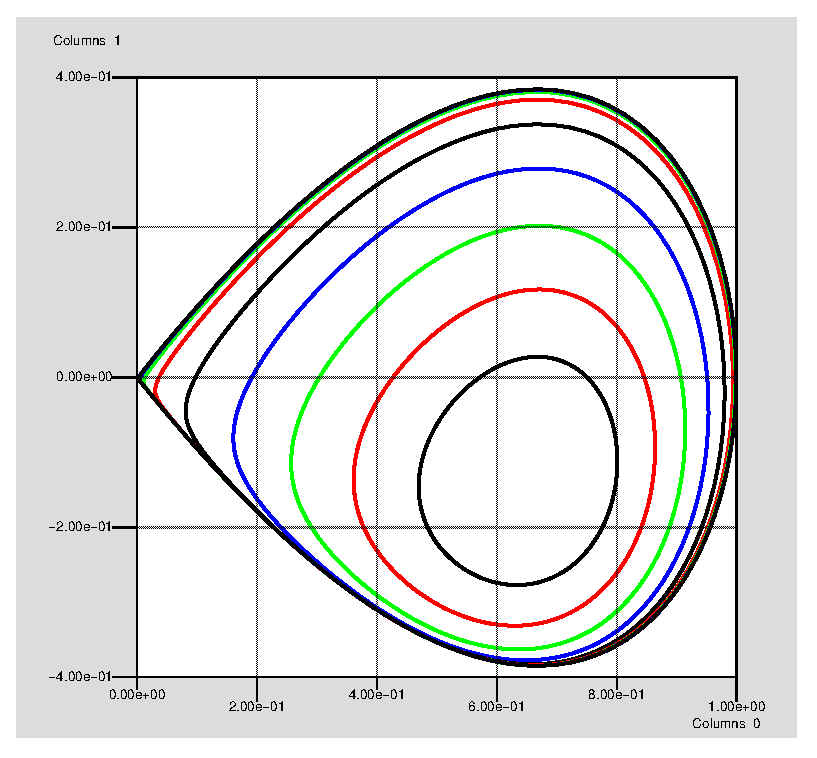
\includegraphics[scale=0.5]{include/hopfbif.eps}}
\put(200,0){
\put(157,148){(b)}
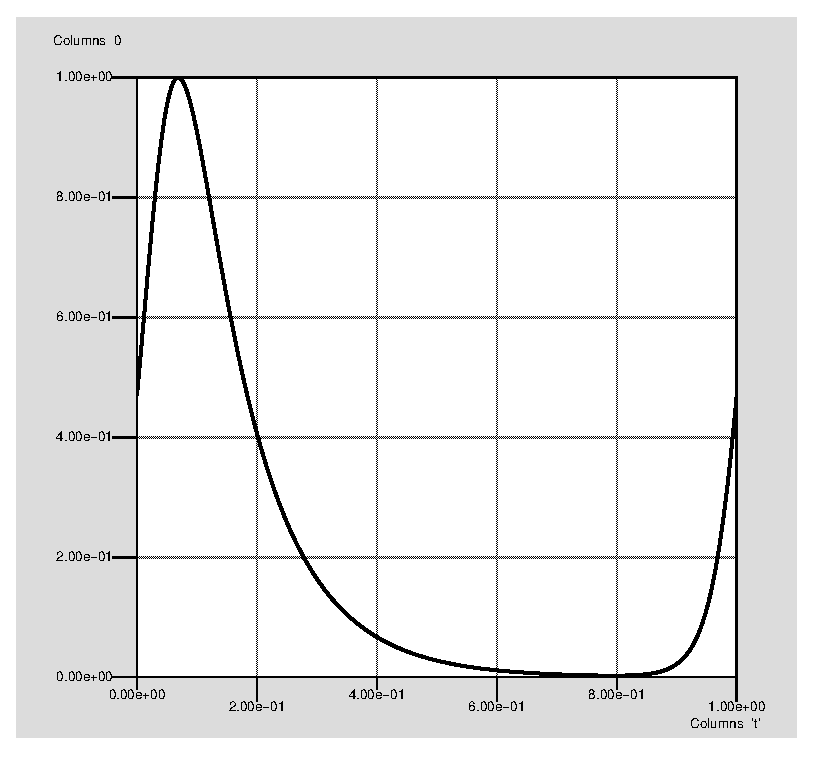
\includegraphics[scale=0.5]{include/notshifted.eps}}
\end{picture}
\caption{Periodic orbit growing from a Hopf bifurcation to a
  homoclinic orbit (a). The unshifted homoclinic orbit (b).}
\label{hopfbif}
\end{center}
\end{figure}

Note however, that the homoclinic orbit has the wrong left-hand and
right-hand end points. This can be seen by plotting the solution
corresponding to Label [13] using 't' vs. 'x' (coordinate [0]), 
as depicted in Figure~\ref{hopfbif}(b).

Hence, in order to continue this as a real homoclinic 
we have to give {\cal HomCont} special instructions, to do a phase-shift in
time. This can be done by setting \parf{ISTART=4}. Moreover, 
since we have not specified the value of
the equilibrium at the origin in \filef{ sib.c}, 
we need to set \parf{IEQUIB=1} to let
{\cal HomCont} detect the equilibrium. Note that in this case this is not
strictly necessary; however, we do this for instructional purposes.

Now we use {\cal HomCont} to continue the homoclinic orbit in $c$ and $\mu$ 
(\parf{PAR(3)}, \parf{PAR(5)}), to get the desired value $c=-2.0$.
\begin{center}
\commandf{ rn(c='sib.4',h='sib.shift',s='3') } \\
\commandf{ sv('4') }
\end{center}
\begin{verbatim}
  BR    PT  TY LAB    PAR(3)        L2-NORM       ...    PAR(5)     
   3    15  EP  14 -2.000000E+00  4.018899E-01    ...  2.661459E-09
\end{verbatim}
The output is saved in the files \filef{ b.4}, \filef{ s.4} and
\filef{ d.4}. Note that \parf{PAR(5)}=$\mu$ remains zero, which is exactly
what we expect.

Next we want to add a solution to the adjoint equation to this
solution. This is achieved by making the change \parf{ ITWIST = 1}
saved in \filef{ h.sib.twist}. Also, we set \parf{ISTART} to 1 to tell 
{\cal HomCont} that it is should not try to shift the orbit anymore.
\begin{center}
\commandf{ rn(c='sib.5',h='sib.twist',s='4') } \\
\commandf{ sv('5') }
\end{center}
or, alternatively,
\begin{center}
\commandf{ cc("IRS",14) }\\
\commandf{ cc("ICP",[5,8])}\\
\commandf{ cc("NMX",2)}\\
\commandf{ chc("ITWIST",1)}\\
\commandf{ chc("ISTART",1)}\\
\commandf{ rn(s='4')}\\
\commandf{ sv('5')}
\end{center}
where \commandf{chc} means ``change {\cal HomCont} constant''.
The output is stored in \filef{ b.5}, \filef{ s.5}  and \filef{ d.5}.
\begin{verbatim}
  BR    PT  TY LAB    PAR(5)         L2-NORM    ...     PAR(8)     
   3     2  EP  15   2.550843E-09  4.018898E-01 ...  -1.000000E-02
\end{verbatim}
Here \parf{PAR(8)} is a dummy (unused) parameter and $\mu$ just stays where
it is. Now that we have obtained the solution of the adjoint equation,
we are able to detect inclination flips. This can be achieved by
setting \parf{NPSI} to 1, \parf{IPSI(1)} to 13, and monitoring \parf{PAR(32)}.
\begin{center}
\commandf{ rn(c='sib.6',h='sib.if',s='5') } \\
\commandf{ sv('6') }
\end{center} 
\begin{verbatim}
  BR    PT  TY LAB    PAR(4)        L2-NORM     ...     PAR(5)        PAR(32) 
   3    11  UZ  16  7.117745E-02  4.018899E-01  ...   1.243774E-11 -2.366987E-07
\end{verbatim}   
The output is stored in \filef{ b.6}, \filef{ s.6}  and \filef{ d.6}.
Hence an inclination flip was found at $\alpha=0.7117745$.

Now we are ready to perform homoclinic branch switching, using
the techniques described in \cite{OlChKr:02}. 
Our first aim is to find a 2-homoclinic orbit. The
ingredients we need are: a homoclinic orbit where $n$-homoclinic orbits
are close by, and the solution to the adjoint equation to
obtain the Lin vector. Since both ingredients are there, we can now
continue in $\mu$, $\varepsilon_1$ and $T_1$, to obtain the initial
Lin gap. Recall from Chapter~\ref{ch:HomCont} that the Lin gaps 
$\varepsilon_i$ correspond to
\parf{PAR(19+i*2)} and the time intervals $T_i$ 
correspond to \parf{PAR(20+i*2)}. We stop when
$\varepsilon_1=0.2$. We need to specify \parf{ITWIST=2}, to tell 
{\cal HomCont} we
aim to find a 2-homoclinic orbit, so that it will split it up in three
parts with two potential Lin gaps. We effectively have a 9-dimensional
system at this point.
\begin{center}
\commandf{ rn(c='sib.7',h='sib.hbs2',s='6') } \\
\commandf{ sv('7') }
\end{center} 
\begin{verbatim}
  BR    PT  TY LAB    PAR(20)       L2-NORM     ...     PAR(21)       PAR(5)
   3    10      18  3.458968E+01  4.468176E-01  ...   7.877123E-07 -1.558861E-11
   3    20      19  2.736992E+01  4.468176E-01  ...   2.911187E-05 -1.639739E-09
   3    30      20  1.737196E+01  4.468171E-01  ...   4.422734E-03 -3.101671E-05
   3    38  EP  21  1.014512E+01  4.467963E-01  ...   2.000000E-01 -1.486151E-02
\end{verbatim}
The output is stored in \filef{ b.7}, \filef{ s.7}  and \filef{ d.7}.
Here we see that $T_1$, the time it takes to make the first loop with
respect to the Poincar\'e section, decreases. This is illustrated in
Figure~\ref{broken}. Next we are ready to close this gap, by continuing
in $\alpha$, $\mu$, and $\varepsilon_1$, while keeping $T_1$ at a
constant value.
\begin{figure}[htb]
\begin{center}
\begin{picture}(400,180)
\put(0,0){
\put(157,148){(a)}
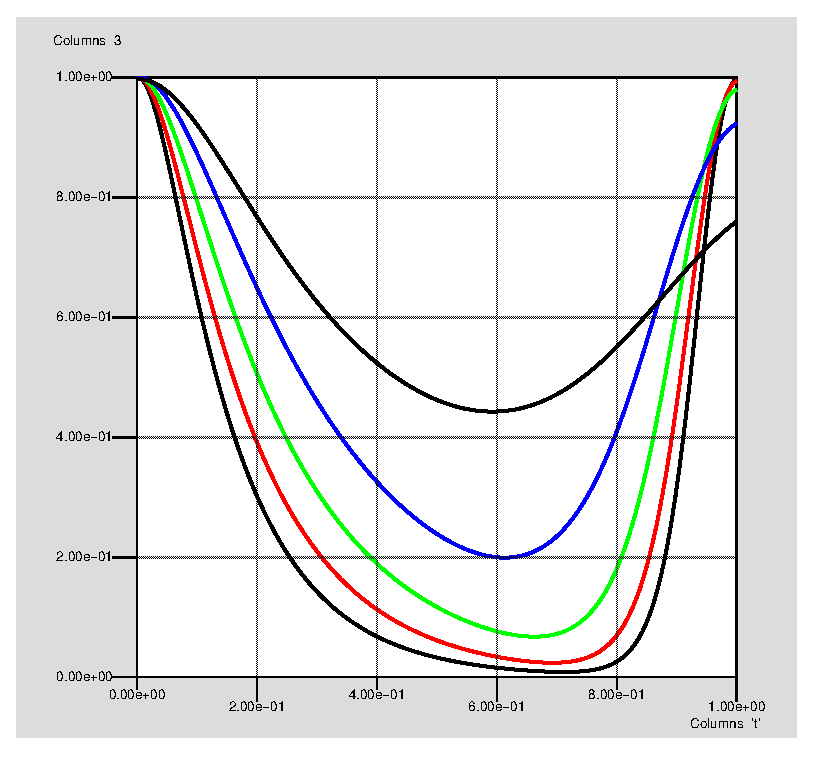
\includegraphics[scale=0.5]{include/loop.eps}}
\put(200,0){
\put(157,148){(b)}
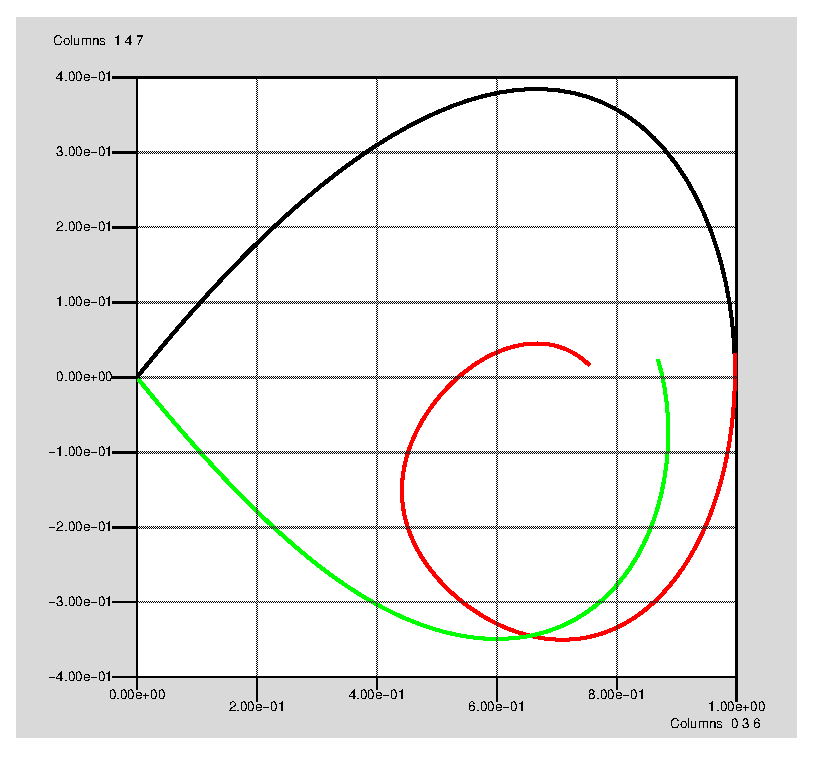
\includegraphics[scale=0.5]{include/broken.eps}}
\end{picture}
\caption{Behaviour of the second piece of the
`broken homoclinic orbit' when creating a Lin gap (a).
Projection of the ``broken homoclinic orbit''
onto the $(x,y)$-plane, where $\varepsilon_1=0.2$. To include all the
pieces necessary to obtain this
figure, the ``X'' box must contain [0,3,6] and the ``Y'' box must contain
[1,4,7] (b).}
\label{broken}
\end{center}
\end{figure}
\begin{center}
\commandf{ rn(c='sib.8',h='sib.hbs2',s='7') } \\
\commandf{ ap('6') }
\end{center} 
\begin{verbatim}
  BR    PT  TY LAB    PAR(4)        L2-NORM     ...     PAR(5)        PAR(21) 
   3     3  UZ  22  7.399999E-02  4.467807E-01  ...  -1.431624E-02  1.937464E-01
   3    32  EP  23  1.992281E-01  4.465901E-01  ...  -6.054949E-03  2.292996E-06
\end{verbatim}
The output is appended to \filef{ b.6}, \filef{ s.6}  and \filef{  d.6}.
Now we have obtained a 2-homoclinic orbit at label 24. However, the
homoclinic orbit is still split in three parts. We can switch back to
a normal orbit by setting \parf{ITWIST} back to 0 and continuing in the usual
way. Here we continue back to the inclination flip point in $\alpha$
and $\mu$.
\begin{center}
\commandf{ rn(c='sib.8',h='sib.hom',s='6') } \\
\commandf{ ap('6') }
\end{center} 
\begin{verbatim}
  BR    PT  TY LAB    PAR(4)        L2-NORM     ...     PAR(5)
   3     7  UZ  24  1.499999E-01  4.944903E-01  ...  -3.602482E-03
   3    30  EP  25  7.614033E-02  4.987463E-01  ...  -2.648395E-06
\end{verbatim}
So the 2-homoclinic orbit converges back to the 1-homoclinic orbit at
the inclination flip bifurcation.
The output is appended to \filef{ b.6}, \filef{ s.6}  and \filef{  d.6}.
The resulting 2-homoclinic orbits can be seen using
\begin{center}
\commandf{ plot('6') }
\end{center} 
and is depicted in Figure~\ref{hom2.eps}(a).
\begin{figure}[htb]
\begin{center}
\begin{picture}(400,180)
\put(0,0){
\put(157,148){(a)}
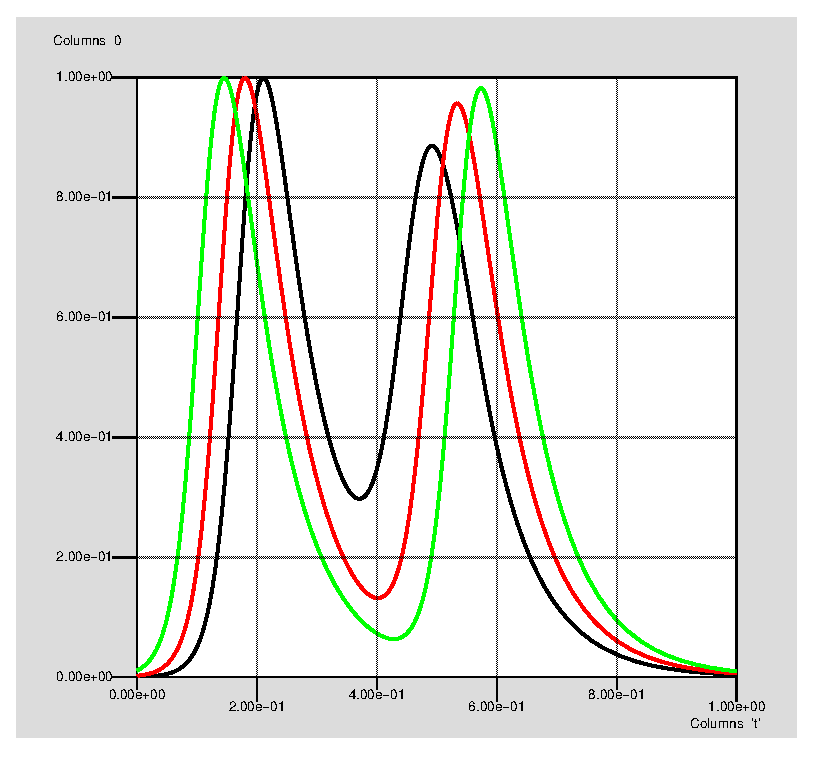
\includegraphics[scale=0.5]{include/hom2.eps}}
\put(200,0){
\put(157,148){(b)}
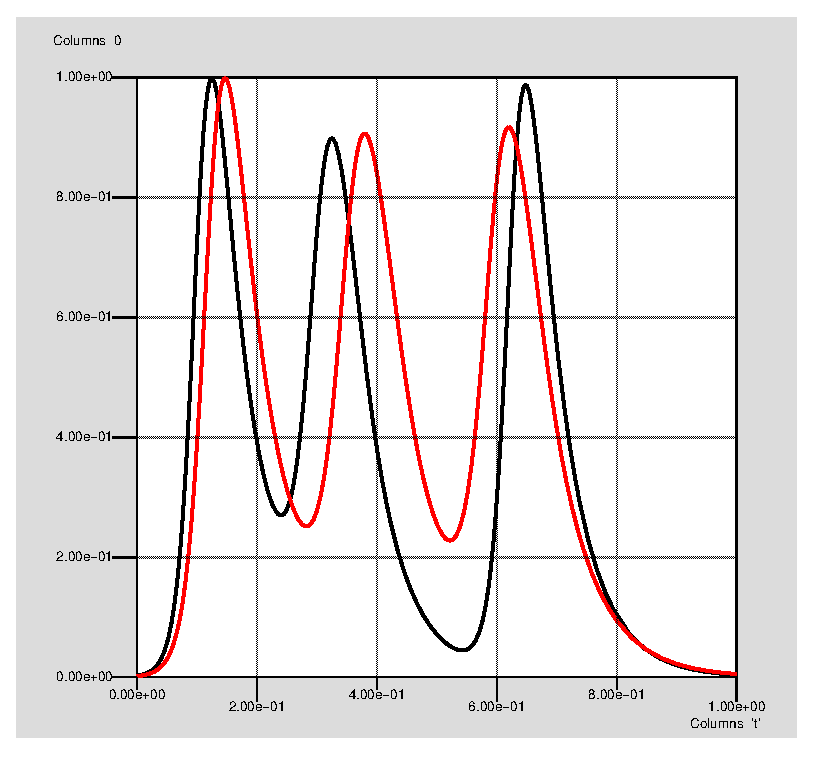
\includegraphics[scale=0.5]{include/hom3.eps}}
\end{picture}
\caption{The 2-homoclinic orbit as $a$ is changed (a).
The two different 3-homoclinic orbits (b).}
\label{hom2.eps}
\end{center}
\end{figure}

Next, we aim to find a 3-homoclinic orbit. To do so, we
restart at the inclination flip point at label 16 and set
\parf{ITWIST=3}. Moreover, we need to continue in one more
gap, $\varepsilon_2$=\parf{PAR(23)} and, once again, stop
when $\varepsilon_1$=\parf{PAR(21)=0}.2. Note that the 
dimension of the boundary value problem we continue
is now equal to 12. This is not to be confused with the setting
of \parf{NDIM=3} in the parameter file, because {\cal HomCont} handles this
internally.
\begin{center}
\commandf{ rn(c='sib.10',h='sib.hbs3',s='6') } \\
\commandf{ sv('10') }
\end{center} 
\begin{verbatim}
  BR    PT  TY LAB    PAR(20)     ...   PAR(21)       PAR(23)       PAR(5)
   3    10      26  3.458963E+01  ... 7.878940E-07  6.421573E-07 -1.062630E-11
   3    20      27  2.736987E+01  ... 2.911260E-05  6.515911E-07 -1.636554E-09
   3    30      28  1.737189E+01  ... 4.422894E-03  1.440898E-04 -3.101882E-05
   3    38  EP  29  1.014512E+01  ... 2.000000E-01  6.974453E-02 -1.486151E-02
\end{verbatim}
The output is stored in \filef{ b.10}, \filef{ s.10}  and \filef{ d.10}.
Now we need to subsequently close the Lin gaps. Our strategy is to
keep $T_1$ fixed. We first continue in $\alpha$, $\mu$,
$\varepsilon_1$ and $\varepsilon_2$ until $\varepsilon_1=0$.
\begin{center}
\commandf{ rn(c='sib.11',h='sib.hbs3',s='10') } \\
\commandf{ ap('6') }
\end{center} 
\begin{verbatim}
  BR    PT  TY LAB    PAR(4)      ...    PAR(5)        PAR(21)       PAR(23)    
   3     6  UZ  30  8.199998E-02  ... -1.297904E-02  1.769949E-01  6.371836E-02
   3    32  EP  31  1.984145E-01  ... -6.054949E-03  2.307164E-06  3.624489E-02
\end{verbatim}
The output is appended to \filef{ b.6}, \filef{ s.6}  and \filef{ d.6}.
Note that this continuation is very similar to the one where we found
a 2-homoclinic orbit. In fact we have now found a 2-homoclinic orbit
(numerically) followed by a `broken' 1-homoclinic orbit; only the mesh
is not aligned.

The next step is to close the gap corresponding to $\varepsilon_2$ to
obtain a 3-homoclinic orbit. We replace the continuation parameter
$\varepsilon_1$ by $T_2$, because $T_2$ (\parf{PAR(22)})
still has to be decreased from
its high value (35) and $\varepsilon_1$ needs to stay at 0.
\begin{center}
\commandf{ rn(c='sib.12',h='sib.hbs3',s='6') } \\
\commandf{ ap('6') }
\end{center} 
\begin{verbatim}
  BR    PT  TY LAB    PAR(4)      ...    PAR(5)        PAR(22)       PAR(23)    
   3    16  UZ  32  1.983953E-01  ... -6.055361E-03  2.013107E+01  1.824909E-08
   3    24  UZ  33  1.800000E-01  ... -6.502928E-03  1.275539E+01 -3.142935E-02
   3    30  UZ  34  1.669900E-01  ... -6.892692E-03  9.417449E+00 -1.031790E-06
   3    32  EP  35  1.781716E-01  ... -6.553641E-03  9.502999E+00 -7.203666E-02
\end{verbatim}
The output is appended to \filef{ b.6}, \filef{ s.6}  and \filef{ d.6}.
Note that we have found two zeros of \parf{PAR(23)}, at labels 32 and
34, respectively. The two zeros
correspond to two different 3-homoclinic
orbits, which, when followed from periodic orbits, both emanate from
from the same saddle-node bifurcation.
These two 3-homoclinic orbits are depicted in Figure~\ref{hom2.eps}(b).
We can follow both of these back to the inclination flip point, by
setting \parf{ITWIST} back to 0:
\begin{center}
\commandf{ rn(c='sib.13',h='sib.hom',s='6') } \\
\commandf{ ap('6') }
\end{center} 
\begin{verbatim}
  BR    PT  TY LAB    PAR(4)        L2-NORM     ...    PAR(5)     
   3    13  UZ  36  1.299993E-01  5.048071E-01  ... -2.339037E-03
   3    30  EP  37  9.272363E-02  5.065599E-01  ... -2.767140E-04
\end{verbatim}
\begin{center}
\commandf{ rn(c='sib.14',h='sib.hom',s='6') } \\
\commandf{ ap('6') }
\end{center}
\begin{verbatim}
  BR    PT  TY LAB    PAR(4)        L2-NORM     ...    PAR(5)     
   3     4  UZ  37  1.449997E-01  5.473471E-01  ... -4.794005E-03
   3    30  EP  39  8.394009E-02  5.526047E-01  ... -7.367526E-05
\end{verbatim}
All the output is appended to \filef{ b.6}, \filef{ s.6}  and \filef{  d.6}.
The bifurcation diagram and the paths we followed when closing the Lin
gaps are depicted in Figure~\ref{parspace}. It is possible and
straightforward to obtain $4, 5, 6, \dots$-homoclinic orbits by 
extending the above strategy.
\begin{figure}[htb]
\begin{center}
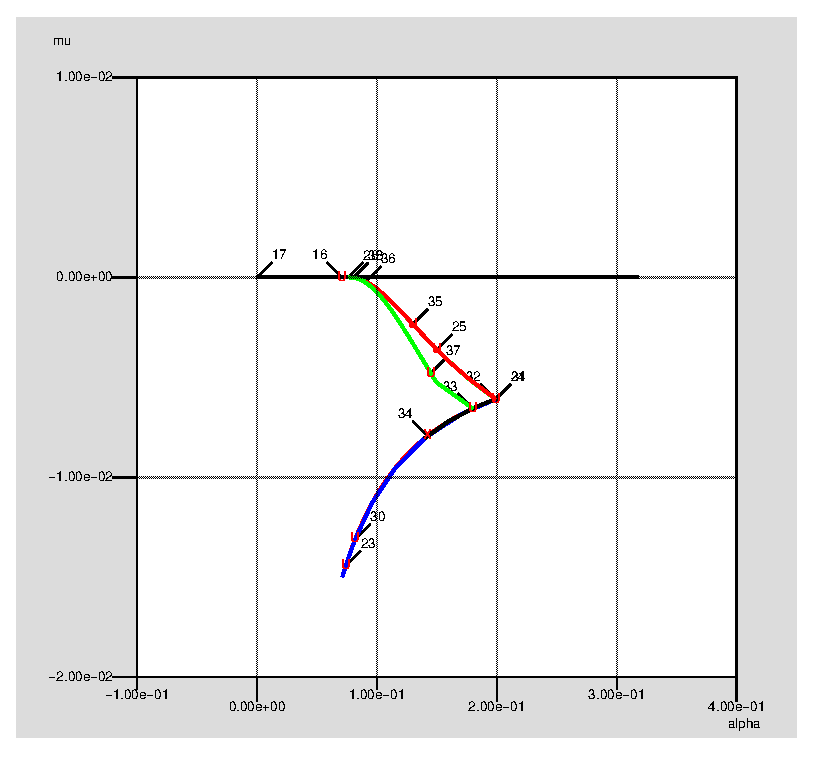
\includegraphics[scale=0.5]{include/parspace.eps}
\caption{Parameter space diagram near an inclination flip. 
The curve
through label 17 corresponds to a 1-homoclinic orbit. 
The opening of the Lin gaps occurs along the vertical line from
label 16 to label 23. The curves
through labels 23 and 30 denote the path that is followed when
closing the Lin gaps. The (approximately overlaid)
curves though labels 25 and 35 correspond to the 
2- and one of the 3-homoclinic orbits.
Finally, the curve through label 37 corresponds to the other
3-homoclinic orbit, which was obtained for \parf{PAR(22)}=$T_2=12.03201$.}
\label{parspace}
\end{center}
\end{figure}

\section{ Branch switching for a Shil'nikov type homoclinic orbit in
the FitzHugh-Nagumo equations.}

The FitzHugh-Nagumo (FHN) equations \cite{FitzH:61,NaArYo:62} 
are a simplified version of the
Hodgkin-Huxley equations \cite{HoHu:52}. 
They model nerve axon dynamics and are given by

\begin{equation}
\begin{split}
u_t&=u_{xx}-f_a(u)-w, \\
w_t&=\epsilon(u-\gamma w),
\end{split}
\label{fhnpde}
\end{equation}
where
\[
f_a(u) = u (u-a)(u-1).
\]

Travelling wave solutions of the form $(u,w)(x,t)=(u,w)(\xi)$, where
$\xi=x+ct$ are solutions of the following ODE system:

\begin{equation}
\begin{split}
\dot u &= v,\\
\dot v &= c v + f_a(u) + w,\\
\dot w &= \frac{\epsilon}{c} (u - \gamma w).
\end{split}
\label{fhnode}
\end{equation}
In particular we consider solitary wave solutions of \eqref{fhnpde}.
These correspond to orbits homoclinic to $(u,v,w)=0$ in system \eqref{fhnode}.
In our numerical example we keep $\gamma=0$.

We aim to find a $2$-homoclinic orbit at a Shil'nikov bifurcation.
All the commands given here are in the file fnb.auto.
First we obtain a homoclinic orbit using a homotopy technique (see
\citeasnoun{FrDoMo:94}), using \parf{ISTART=3}, for the parameter 
values $c=0.21, a=0.2, \epsilon=0.0025$.

\begin{center}
\commandf{ demo('sib') }\\
\commandf{ld('fnb')}\\
\commandf{rn()}\\
\commandf{sv('1')}
\end{center}

Among the output we see:
\begin{verbatim}
  BR    PT  TY LAB     PERIOD       L2-NORM     ...     PAR(16)    
   1    20  UZ   3  2.922565E+01  2.379162E-01  ...  -1.680003E-09
\end{verbatim}
and a zero of \parf{PAR(16)} means that a zero of an artificial parameter has
been located and the right-hand end point of the corresponding
solution belongs to the plane that is tangent to the stable manifold
at the saddle. This point still needs to come closer to the
equilibrium, which we can achieve by further increasing the period to
300, while keeping \parf{PAR(16)} at 0:
\begin{center}
\commandf{rn(c='fnb.2',h='fnb.1',s='1')}\\
\commandf{sv('2')}
\end{center}
\begin{verbatim}
  BR    PT  TY LAB     PERIOD       L2-NORM     ...    PAR(1)     
   1   190  UZ  10  3.000000E+02  7.379317E-02  ...  1.792864E-01
\end{verbatim}

Next we stop using the homotopy technique and increase the period even
further, to 1000.
\begin{center}
\commandf{rn(c='fnb.3',h='fnb.3',s='2')}\\
\commandf{sv('3')}
\end{center}
\begin{verbatim}
  BR    PT  TY LAB     PERIOD       L2-NORM     ...    PAR(1)     
   1    80  UZ  13  1.000000E+03  4.041827E-02  ...  1.792865E-01
\end{verbatim}

A continuation in \parf{PAR(1)}=$a$ and \parf{PAR(0)}=$c$ needs to be 
performed to arrive
at the place where we wish to find a 2-homoclinic orbit: $a=0$. At the
same time we monitor \parf{PAR(21)} to locate Belyakov points.
\begin{center}
\commandf{rn(c='fnb.4',h='fnb.4',s='3')}\\
\commandf{sv('4')}
\end{center}
\begin{verbatim}
  BR    PT  TY LAB    PAR(1)        L2-NORM     ...    PAR(0)        PAR(21)  
   1     6  UZ  15  1.318124E-01  3.287104E-02  ...  2.171656E-01 -6.312189E-06  
   1    23  UZ  19 -8.545741E-08  1.561579E-02  ...  2.742181E-01 -9.887718E-02
\end{verbatim}
Hence, there exists a Belyakov point at $(a,c)=(0.1318124,0.217656)$.
At label 19 we have a lower value of $a$ than at the Belyakov point,
and by inspection of the file
\filef{d.4} we can observe that the equilibrium has one positive
eigenvalue and a complex conjugate pair of eigenvalues with negative
real part, and conclude that this orbit is of Shil'nikov type.
Before starting the homoclinic branch switching, we calculate
the adjoint to obtain a `Lin vector':
\begin{center}
\commandf{rn(c='fnb.5',h='fnb.5',s='4')}\\
\commandf{sv('5')}
\end{center}
\begin{verbatim}
  BR    PT  TY LAB    PAR(8)        L2-NORM     ...    PAR(2)     
   1     2  EP  28 -1.000000E+00  1.561579E-02  ...  2.500000E-03
\end{verbatim}
Next, we continue in the time $T_1$ (\parf{PAR(20)}), the gap
$\varepsilon_1$ (\parf{PAR(21)}) and $c$ (\parf{PAR(0)}), 
and by setting \parf{ISTART}=-2
we try to locate a 2-homoclinic orbit:
\begin{center}
\commandf{rn(c='fnb.6',h='fnb.6',s='5')}\\
\commandf{sv('6')}
\end{center}
In fact we find many of them, exactly as is predicted by the theory:
\begin{verbatim}
  BR    PT  TY LAB    PAR(20)     ...    PAR(0)        PAR(21)   
...
   1   175  UZ  45  1.647952E+02  ...  2.742181E-01 -2.313522E-11
   1   179  UZ  46  1.448063E+02  ...  2.742181E-01  1.481383E-11
   1   183  UZ  47  1.248379E+02  ...  2.742181E-01  2.171338E-16
   1   188  UZ  48  1.048192E+02  ...  2.742181E-01  5.215295E-11
   1   192  UZ  49  8.487422E+01  ...  2.742181E-01  3.106887E-15
   1   197  UZ  50  6.463349E+01  ...  2.742181E-01 -1.803730E-10
\end{verbatim}
Each of these homoclinic orbits differ 
by about 20 in the value $T_1$. This is about 
the time it takes to make one half-turn close to and
around the equilibrium, so that orbits differ by the number of 
half turns around the equilibrium before a big excursion
in phase space. Note that the variation of 
$c$ is so small that it does not appear.

A plot of $T_1$ vs. $\varepsilon_1$ gives insight into how the gap
is opened and closed in the continuation process. This is depicted in 
Figure~\ref{shilgap}.
\begin{figure}[htb]
\begin{center}
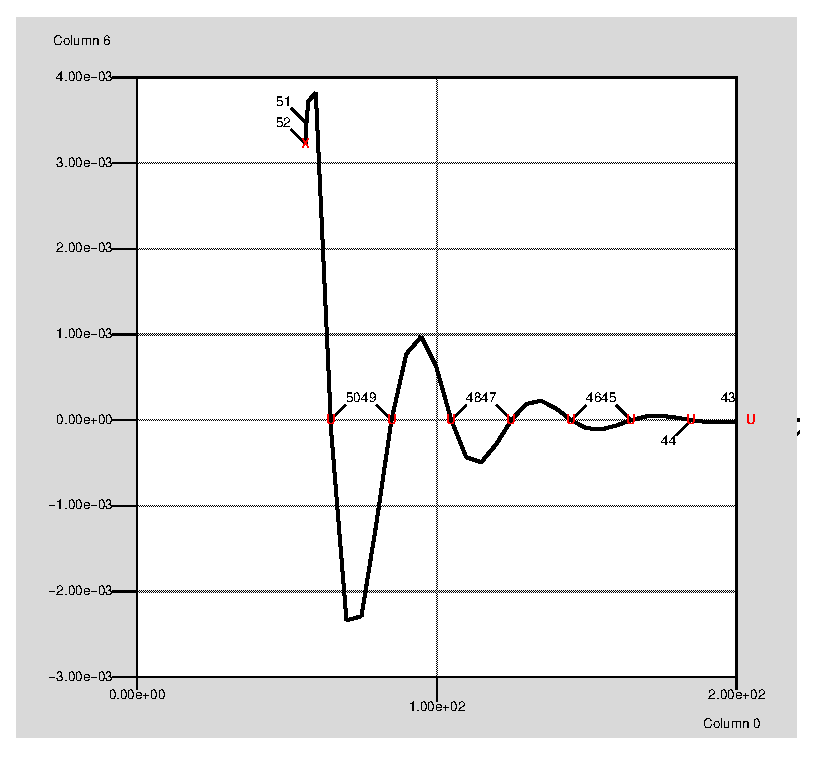
\includegraphics[scale=0.5]{include/shilgap.eps}
\caption{A plot of $\varepsilon_1$ as a function of $T_1$ 
during our computation of Shil'nikov-type two-homoclinic orbits. 
Each zero corresponds to a different orbit.}
\label{shilgap}
\end{center}
\end{figure}
We are now in a
position to continue each of these orbits as a
normal homoclinic orbit by setting \parf{ISTART=1} and
\parf{ITWIST=0}. We leave
this as an exercise to the reader.

\section{ Branch switching to a 3-homoclinic orbit in
a\\ 5th-order Korteweg-De Vries model}

In \citeasnoun{ChGr:97} the following water wave model was considered:
\begin{equation}
\frac{2}{15}r''''-b r''+ar+\frac{3}{2}r^2-
\frac{1}{2}(r')^2+[rr']' = 0.
\label{cgode}
\end{equation}
It represents solitary-wave solutions $r(x+at)$, $r\to 0$ as $x\to
\pm\infty$ of the 5th-order PDE
\[
r_t+\frac{2}{15}r_{xxxx}-b r_{xxx}+3r r_x+2 r_x r_{xx}+r r_{xxx=0},
\]
where $a$ is the wave speed.
The ODE corresponds to a Hamiltonian system with Hamiltonian
\[ H=-\frac{1}{2}q_1^3-\frac{1}{2}a q_1^2+p_1 q_2-\frac{1}{2}b q_2^2+
\frac{15}{4}p_2^2+\frac{1}{2}q_2^2 q_1 \]
and 
\[q_1=r, \quad q_2=r', \quad p_1=-\frac{2}{15}r'''+br'-rr', \quad p_2=\frac{2}{15}r''.\]
System \eqref{cgode} is also reversible under the transformation 
\[ t \mapsto -t, (q_1,q_2,p_1,p_2)\mapsto (q_1,-q_2,-p_1,p_2),\] 
but we do not exploit the reversible structure (\parf{IREV=0}), and
instead use it as an example of Hamiltonian system.
This system exhibits an orbit flip for a reversible Hamiltonian system.
In Hamiltonian systems, homoclinic orbits are codimension-zero
phenomena, and we have to add an additional parameter $\lambda$ that breaks
the Hamiltonian structure in this system, by introducing artificial friction.
Thus, the actual system of equations that is
used for continuation is
\[\dot x=(\lambda I + J)\nabla H(x),\]
where $x=(q_1,q_2,p_1,p_2)$ and $J$ is the usual skew symmetric matrix
in $\mathbb{R}^4$.
It is now possible to continue a homoclinic orbit in {\cal HomCont} in two
parameters ($\lambda$ and either $a$ or $b$); see also
\citeasnoun{Be:90a}.

An explicit solution exists for $a=3/5(2b+1)(b-2), b\geq -1/2$, and it is
given by 
\[r(t)=3(b+\frac{1}{2})\mathrm{sech}^2\left([\frac{3}{4}(2b+1)]^{1/2}t\right).\]
It corresponds to a reversible orbit flip for $b>2$ ($a>0$) 
We start from this explicit solution, using \parf{ISTART=2}, for $a=3$ and
$b=(\sqrt{65}+3)/4$:

\begin{center}
\commandf{demo('kdv') }\\
\commandf{ld('kdv')}\\
\commandf{rn()}\\
\commandf{sv('1')}
\end{center}
\begin{verbatim}
  BR    PT  TY LAB    PAR(0)        L2-NORM     ...    PAR(2)     
   1     1  EP   1  3.000000E+00  5.565438E+00  ...  0.000000E+00
   1     2  EP   2  3.049592E+00  5.491407E+00  ...  1.807155E-17
\end{verbatim}
Here \parf{PAR(0)}=$a$, \parf{PAR(1)}=$b$, and
\parf{PAR(2)}=$\lambda$. We have only done a
very small continuation to give \AUTO a chance to create a good mesh
and avoid convergence problems later.
Next, we set \parf{ITWIST=1} and calculate the adjoint:
\begin{center}
\commandf{rn(c='kdv.2',h='kdv.2',s='1')}\\
\commandf{sv('2')}
\end{center}
\begin{verbatim}
  BR    PT  TY LAB    PAR(1)        L2-NORM     ...    PAR(8)     
   1     2  EP   3  2.765575E+00  5.491418E+00  ... -6.250114E-04
\end{verbatim}
We now need to move back to the orbit flip at $a=3$:
\begin{center}
\commandf{rn(c='kdv.3',h='kdv.3',s='2')}\\
\commandf{sv('3')}
\end{center}
\begin{verbatim}
  BR    PT  TY LAB    PAR(0)        L2-NORM     ...    PAR(2)     
   1    14  UZ   5  3.000000E+00  5.476133E+00  ...  1.483821E-09
\end{verbatim}
Now all preparations are done to start homoclinic branch
switching. This is very similar to the technique used in 
Sandstede's model in Section~\ref{sec:HomCont_hbs_san}; 
to find a 3-homoclinic orbit, we open 2 Lin gaps,
until $T_1=3.5$, while also varying $\lambda$=\parf{PAR(2)}.
\begin{center}
\commandf{rn(c='kdv.4',h='kdv.4',s='3')}\\
\commandf{sv('4')}
\end{center}
\begin{verbatim}
  BR    PT  TY LAB    PAR(2)      ...    PAR(20)       PAR(21)       PAR(23)  
   1    10       8  5.797610E-10  ...  1.672717E+01 -8.381610E-08 -6.988443E-07
   1    19  UZ   9  1.399137E-09  ...  1.012493E+01  6.452744E-12  1.379764E-07
   1    20      10  2.122922E-09  ...  9.001030E+00  1.032750E-07  4.022729E-07
   1    29  EP  11  2.154196E-06  ...  3.499999E+00  7.959776E-04  3.999453E-04
\end{verbatim}
We then look for an orbit with $a<3$ and close the gap corresponding 
to $\varepsilon_1$=\parf{PAR(21)}, for decreasing $a$.
\begin{center}
\commandf{rn(c='kdv.5',h='kdv.5',s='4')}\\
\commandf{sv('5')}
\end{center}
\begin{verbatim}
  BR    PT  TY LAB    PAR(1)      ...    PAR(2)        PAR(21)       PAR(23)       
   1    10      12  2.579042E+00  ...  2.154861E-06  7.659464E-04  3.829183E-04  
   1    13  UZ  13  2.320452E+00  ...  3.933752E-11  1.088379E-10  1.552594E-08
   1    20  EP  14 -1.906119E-01  ... -1.022044E-03 -7.600151E-01 -3.446967E-01
\end{verbatim}
and finally close the gap corresponding to $\varepsilon_2$=\parf{PAR(23)},
\begin{center}
\commandf{rn(c='kdv.6',h='kdv.6',s='5')}\\
\commandf{sv('6')}
\end{center}
\begin{verbatim}
  BR    PT  TY LAB    PAR(1)      ...    PAR(2)        PAR(22)       PAR(23)   
   1    23  UZ  15  2.320450E+00  ...  2.198310E-12  1.487623E+01 -4.392295E-10
   1    30      16  2.320380E+00  ... -1.004669E-09  1.027163E+01 -5.060989E-07
   1    51  UZ  17  2.336952E+00  ...  2.374866E-07  3.482932E+00  1.195914E-04
   1    58  UZ  18  3.080847E+00  ...  2.673602E-12  3.500044E+00 -1.934478E-10
   1    60  EP  19  3.134237E+00  ... -5.614124E-07  3.778288E+00 -3.398845E-04
\end{verbatim}
so that a three-homoclinic orbit is found. Here the zero at label
17 is the one we are looking for. Label 15 is a false positive since
$T_2$=\parf{PAR(22)} is still too high. At label 18, $a$=\parf{PAR(1)} 
has changed
considerably to the extend that $a>3$ and a second 3-homoclinic orbit 
is found. Note that for all zeros of \parf{PAR(23)}=$\varepsilon_2$, the
parameter $\lambda$=\parf{PAR(2)} is also zero (within \AUTO accuracy), 
which it has to be to remain
within the original Hamiltonian system.
Setting \parf{ISTART=1}, a normal ``trivial'' continuation (with \parf{NMX=1})
of the orbit corresponding to label 17 
lets {\cal HomCont} produce a proper concatenated
3-homoclinic orbit:
\begin{center}
\commandf{rn(c='kdv.7',h='kdv.7',s='6')}\\
\commandf{sv('7')}
\end{center}
\begin{verbatim}
  BR    PT  TY LAB    PAR(1)        L2-NORM    ...    PAR(2)    
   1     2  EP  20  2.336952E+00  7.505830E+00 ...  2.374866E-07
\end{verbatim}
This 3-homoclinic orbit is depicted in Figure~\ref{kdv3hom}.
\begin{figure}[htb]
\begin{center}
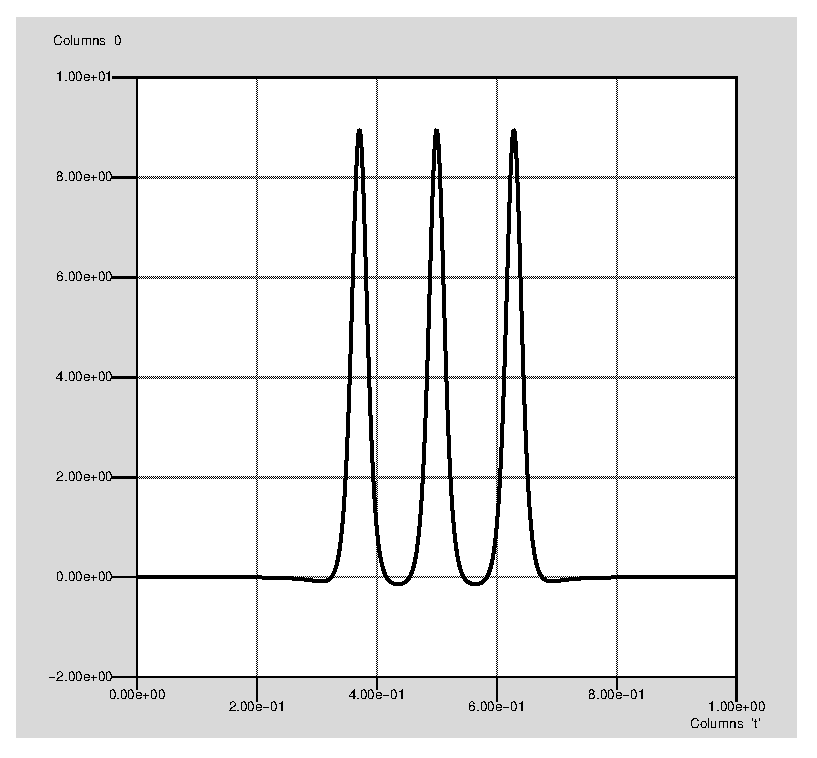
\includegraphics[scale=0.5]{include/kdv3hom.eps}
\caption{A 3-homoclinic orbit in a 5th-order Hamiltonian 
Korteweg-De Vries model.}
\label{kdv3hom}
\end{center}
\end{figure}










